\documentclass{aiaa-tc}% insert '[draft]' option to show overfull boxes

\usepackage{graphicx}
\usepackage{amsmath}
\usepackage{calc}%allows for scaling figures with integer division/multiplication of existing lengths
\usepackage{wrapfig}
\usepackage{lipsum}
\usepackage[hidelinks]{hyperref}
\usepackage{color}
\usepackage{siunitx}
\usepackage{nicefrac}
\usepackage{tikz}
%\usepackage{hyperref}
%\usepackage{biblatex}

\title{Design and Manufacture of an Open-Hardware 
 	University Rocket Airframe using Carbon Fiber}

\author{
Joseph Shields, Leslie Elwood, and Jacob East%, Brandon Bonner, Erik Nelson
	\thanks{Portland State University, Portland, OR 97201}
 }
% Data used by 'handcarry' option if invoked
\AIAApapernumber{2016}
\AIAAconference{SPACE, Sep. 13, Long Beach, California}
\AIAAcopyright{\AIAAcopyrightD{2016}}
\bibliographystyle{aiaa}
 
% Define commands to assure consistent treatment throughout document
\DeclareSIUnit\Far{\degree F}
\DeclareSIUnit\poundF{lb}
\newcommand{\mathregistered}{\text{\textregistered}}
\newcommand{\eqnref}[1]{(\ref{#1})}
\newcommand{\class}[1]{\texttt{#1}}
\newcommand{\package}[1]{\texttt{#1}}
\newcommand{\file}[1]{\texttt{#1}}
\newcommand{\BibTeX}{\textsc{Bib}\TeX}
\newcommand{\cots}{commercial off-the-shelf}
\newcommand{\weightReduction}{80\%}
\newcommand{\strengthIncrease}{??\%}

\begin{document}
\maketitle
% Hello

\begin{abstract}
The amateur and university rocketry communities are rapidly reaching higher altitudes with more sophisticated rockets. However, most groups are still using heavy airframes made of metal or fiberglass. Commercial off-the-shelf airframes are either too expensive for low-budget university groups or too small to use as a platform for high altitude experiments. 
A capstone team of mechanical engineering seniors at Portland State University has developed a low-weight, modular carbon fiber airframe as an open-hardware technology for university rocketry. 
This project continues the work of a 2014 capstone team, who developed a carbon fiber layup process with promising results. 
This will enable low-budget groups like the Portland State Aerospace Society to explore high altitude science and compete in the university space race.  \end{abstract}

\section*{Nomenclature}
\begin{itemize}
	\item CFD, Computational Fluid Dynamics
	\item PSAS, Portland State Aerospace Society
	\item LV2, Launch Vehicle 2
	\item LV3, Launch Vehicle 3
	\item HPR, High Power Rocketry
	\item CF, Carbon Fiber
\end{itemize}


\section{Introduction}
%REMEMBER TO SPECIFY ALL ACRONYMS/INITIALISMS!

\begin{wrapfigure}{R}{2.5 in}
\centering
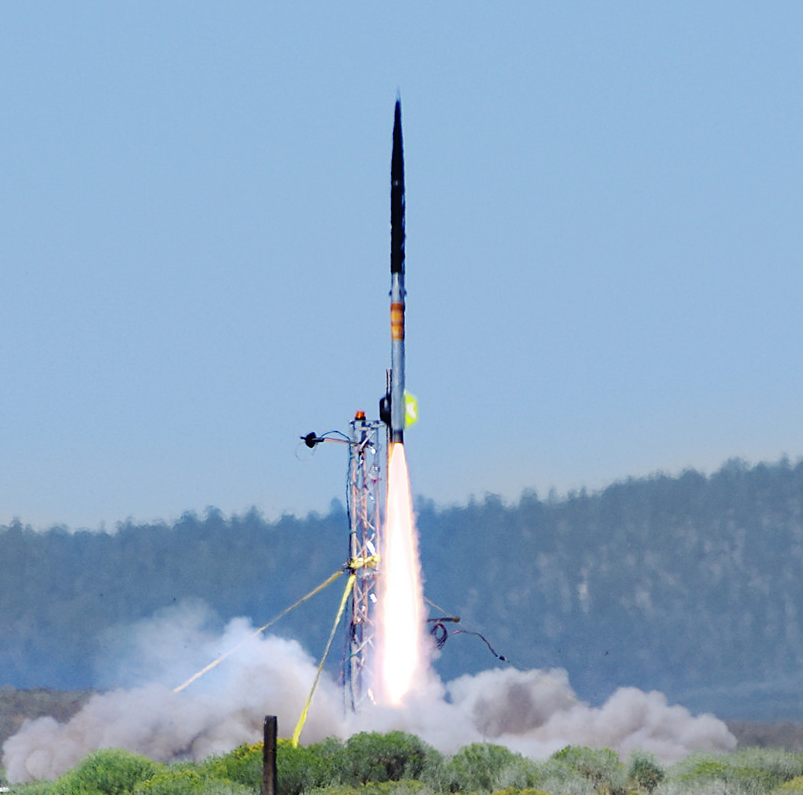
\includegraphics[width=\linewidth]{../img/L12-cropped.png}
\caption{PSAS' LV2 rocket lifting off for the group's $13^\text{th}$launch. The custom cylindrical patch antenna can be seen as a brown band around the middle of the rocket.}
\label{fig:L-12}
\end{wrapfigure}

The Portland State Aerospace Society (PSAS) is an interdisciplinary group of engineering students and alumni of Portland State University (PSU) with the long term goal of putting a cubesat into orbit with their own rocket. 
% info about cubesat market growth: http://www.spaceref.com/news/viewpr.html?pid=44940 
Their current airframe, named Launch Vehicle 2 (LV2), has served for over 12 years, representing 10 of the group's 13 launches, and hosted experiments ranging from custom patch antennas and long range WiFi technology to GPS navigation and a cold gas reaction control system (figure \ref{fig:L-12}). The LV2 platform is mostly constructed of aluminum with a fiberglass shell, with many of the parts having been fabricated in home garages. This makes for a robust but heavy design. Additionally, this airframe is built with a 4.5 inch inner diameter which PSAS's experiments have outgrown. 

The new airframe being designed, named Launch Vehicle 3 (LV3), aims to address these issues. The LV3 platform uses a 6 inch inner diameter, modules composed of carbon fiber and thin aluminum coupling rings, a carbon fiber nose cone, and a carbon fiber fin section. All of the airframe components connect via standardized rings, to accommodate future experimental modules and flight configurations.
The cylindrical LV3 airframe modules outperform the old design with an \weightReduction{} reduction in weight.
% Do we know what the increase in strength is? Also, can we confirm the weight reduction?

\subsection{Basic Design}

The majority of the LV3 airframe uses a sandwich shell composed of CF faces surrounding an aramid honeycomb core (see figure \ref{fig:moduleDiagram}). This provides a rigid structure while minimizing weight. 
Single sheets of carbon fiber are rigid when subjected to in-plane loading, and very flexible in bending. Meanwhile, the core is flexible in bending, and rigid under out-of-plane loading. 
When laminated together, these form a plate which is rigid in all loading conditions. The core material separates the rigid CF faces, greatly increasing the second moment of inertia of the plate. 
There is much more to the theory of sandwich plates and beams, but that is outside the scope of this paper. 

\begin{wrapfigure}{R}{2.5 in}
\centering
\def\svgwidth{\linewidth}
\input{moduleDiagram.pdf_tex}
\caption{Diagram of the male end of a module. The CF (1) is bonded to the honeycomb core (3) and the aluminum coupling ring (4) using structural adhesive (2). The adhesive also serves as a protective coating for the CF and provides a smooth outer surface.}
\label{fig:moduleDiagram}
\end{wrapfigure}

The body of the airframe is composed of modular cylindrical sections using this sandwich design with aluminum coupling rings co-molded to each end.
Each module can hold avionics, experiments, or other equipment with six tapped holes around the inside of the female coupling ring. 
For the radio module, FG takes the place of the CF to allow radio transparency.

The fins use the same sandwich design, with an aluminum frame defining their planform. The center of the frame is filled with core material, and the whole surface is covered in carbon fiber. 
The leading and trailing edges of the fins are made of machined phenolic resin, co-bonded with the frame and CF faces. 
The fins are fins are attached to a module with epoxy fillets, using chopped CF as a filler, and ``tip-to-tip'' CF sheets running from the tip of one fin across the module to the tip of the other fin.

The nose cone uses the same coupling ring system as the modules. It is a von K\'arm\'an ogive formed from two molded CF shells. 
Unlike the rest of the airframe, the nose cone uses a thin shell of two CF sheets, rather than a sandwich design (see section \ref{sec:noseCone} for details). 
The tip of the nose cone is machined out of aluminum and is removed when assembling the recovery system inside the nose cone. 

\subsection{Significance}
Many amateur and university rocketry groups use composite airframes. However, these designs use many layers of fabric, with low fiber volume fractions.
While easy and durable, this does not fully take advantage of their materials. The LV3 design achieves a much higher specific strength and rigidity, enabling greater altitudes with a given motor. 

This design also occupies an uncommon regime for sandwich shell designs. Most such designs use sandwich shells in large, low curvature parts, whereas the LV3 modules have a relatively small size and high curvature.

This is also the only fully open-hardware rocket airframe in the HPR level 3 range. All of the documentation, design, and testing information if freely available on PSAS's Github page \cite{LV3repo}.
%----------need to make extra-sure there aren't any other open-hardware airframes out there----------

\subsection{Software}
\subsubsection{OpenRocket}
For the early design of amateur and university-scale rockets, \href{http://openrocket.sourceforge.net/}{OpenRocket} is very useful. 
It is an open-source Java application which simulates a rocket's flight. It provides a convenient interface for configuring the rocket, selecting commercial or custom parts, viewing the predictions, and performing some basic optimization. 

Using OpenRocket to guide the initial design allowed for rapid iteration of the fin geometry and the placement of non-airframe components. 

\subsubsection{OpenFOAM}
OpenFOAM is another open-source application. It provides a common interface for a wide range of CFD solvers.
Although it requires more up-front effort, it allows a more detailed perspective on what features of an airframe's geometry are the most critical. 
CFD analysis is probably not necessary for most amateur and university level airframe design, but this provides a good option for groups that can't afford a licence for a commercial CFD suite. 

OpenFoam was used to asses the heating at the tip of the nose, to determine if the epoxy matrix of the carbon fiber would degrade over repeated flights.


\section{Materials}

Nearly all of the materials used in the LV3 airframe were donated. The pre-impregnated CF and the structural adhesive were made available after they expired for use in commercial aircraft. 
Acquiring expired materials from large manufacturers and distributors is the strongly preferred over purchasing them outright or simply using cheaper materials. 
Distributors are unlikely to offer these materials in quantities appropriate to this type of project. 
Using non-pre-impregnated CF with painted-on epoxy could change the manufacturing significantly, and would increase the weight of the airframe. 
Acquiring donations is also a good way for university groups to form industry contacts. It can even become an opportunity to collaborate with other university groups, through the re-donation of excess material. 

The CF is a plain weave design that is pre-impregnated with epoxy resin which cures at $\SI{350}{\Far}$.
Meanwhile, the adhesive is an epoxy film which cures between $\SI{250}{\Far}$ and $\SI{350}{\Far}$, intended for bonding metals and composites. 
This allows for co-curing of both materials together. The core material is an over-expanded honeycomb Nomex$^\mathregistered$ mat which bonds well to the adhesive.
Finally, the coupling rings are machined out of 6061-T6 aluminum. 

Any groups obtaining materials through donations will likely not have much control over what materials they get, let alone be able to obtain the exact same materials listed here.
As such, any potential donations should be researched before they are accepted and tested afterwards. 
Any weave of CF will work, through satin is preferred. Pre-impregnated CF should be tacky at room temperature.
Adhesive should either be tacky at room temperature or become tacky when heated. Ideally, it should flow at higher temperatures. 
The core material for the modules should be over-expanded or under-expanded. 
Optimally expanded honeycomb cannot be used for the modules, since it ``potato chips,'' bending away from the module along the axis when it is bent around the circumference. 
The fin core material may use any cell shape and should be $\nicefrac{1}{8}''$ or smaller. 
%---------check what the preferred notation is for length (fractional inches, decimal inches, centimeters...)---------

\subsection{Acquisition}
% Need to change to neutral 3rd person and remove superlatives. 
% Remove informal language like "come aboard"
% Add the appropriate TM/C/R labels to industry names, as per the AIAA style guide. https://www.aiaa-space.org/uploadedFiles/AIAA-Aviation_Site/Footer/AIAA_Paper_Style_Guide.pdf
% Also, I'm not sure we need to go into this much detail for the paper.
The ability to build on a very small budget and further, to donate additional material to other local groups is the epitome of open source. 

Establishing industry relationships benefited our group both for the time being and for PSAS into the future. The largest and most helpful of the material donations made throughout the composite airframe project was made by Boeing. They supplied PSAS with pre-impregnated carbon fiber, Metlbond$^\mathregistered$ 1515-3M structural adhesive, vacuum bagging kits made up of high temperature bagging material, release film, tape, and breather material. Additionally, Boeing also provided professional consulting. Teleconferencing with composite experts from across the nation where made available to us on a weekly basis.  

Pacific Coast Composites (PCC) were the first industry to come aboard. They were able to donate the first roll of pre-impregnated carbon fiber and 3M structural adhesive. PCC also gave PSAS a substantial quantity of both 250°F and 350°F pre-impregnated fiber glass. Portland State University's facilities could not accommodate for all of this material. A small freezer purchased from years before had been totally filled and the rolls of carbon fiber needed to be modified to fit into the small freezer. A much larger freezer was eventually purchased by the Mechanical Engineering department to store the Boeing material. Because the fiber glass was not a priority material, it was stored in the Biology department while we sought other near-by universities. Eventually, Oregon State University and Washington State University inquired about our abundance and we were able to donate the abundance of fiber glass to their aerospace clubs. 


\section{Cylindrical Modules}\label{sec:modules}

Each module has a male coupling ring on the end facing the direction of travel and a female coupling ring on the other end. 
Modules were made in both $18''$ and $24''$ lengths, to accommodate different lengths of motors and equipment. 
By exchanging modules of different lengths, this also allows the overall length of the rocket to be adjusted in increments of $6''$.
The body of the module consists of two concentric CF tubes separated by a honeycomb core, with adhesive bonding the CF to the core and rings (see figure \ref{fig:moduleDiagram}). 
A layer of adhesive also covers the outer layer of CF, serving three roles. First, it ensures the outer layer of CF is completely wetted. 
The pre-impregnated CF used here did not completely wet when cured alone, however this will not be true for every product.
Second, it serves as a protective coating for the CF. 
Third, it can be sanded to improve the surface roughness.
Using a profilometer, the surface features of the uncoated modules was found to be $\SI{179}{\micro\meter}$ ($\SI{7.1e-3}{in}$), while the surface features of the adhesive-coated modules could be sanded to $\SI{3.3}{\micro\meter}$ ($\SI{1.3e-4}{in}$).

\begin{wrapfigure}{R}{2.5 in}
\centering
% Created by tikzDevice version 0.10.1 on 2016-08-17 11:40:13
% !TEX encoding = UTF-8 Unicode
\begin{tikzpicture}[x=1pt,y=1pt]
\definecolor{fillColor}{RGB}{255,255,255}
\path[use as bounding box,fill=fillColor,fill opacity=0.00] (0,0) rectangle (289.08,216.81);
\begin{scope}
\path[clip] ( 48.00, 48.00) rectangle (289.08,204.81);
\definecolor{drawColor}{RGB}{0,0,0}

\path[draw=drawColor,line width= 0.4pt,line join=round,line cap=round] ( 56.93, 63.08) --
	( 57.15, 62.62) --
	( 57.60, 62.31) --
	( 57.94, 61.85) --
	( 58.39, 61.22) --
	( 58.84, 60.61) --
	( 59.18, 60.14) --
	( 59.62, 60.30) --
	( 59.96, 60.46) --
	( 60.40, 60.62) --
	( 60.84, 60.93) --
	( 61.18, 61.24) --
	( 61.62, 61.40) --
	( 62.07, 61.72) --
	( 62.40, 62.03) --
	( 62.84, 62.03) --
	( 63.18, 62.03) --
	( 63.62, 62.04) --
	( 64.07, 61.73) --
	( 64.41, 61.42) --
	( 64.52, 61.26) --
	( 64.64, 60.80) --
	( 64.75, 60.18) --
	( 64.75, 59.55) --
	( 64.87, 59.09) --
	( 64.87, 58.46) --
	( 64.88, 57.84) --
	( 64.88, 57.37) --
	( 65.11, 56.75) --
	( 65.22, 56.44) --
	( 65.33, 55.82) --
	( 65.56, 55.20) --
	( 65.79, 54.73) --
	( 66.24, 54.43) --
	( 66.57, 54.12) --
	( 67.02, 53.81) --
	( 67.46, 54.28) --
	( 67.68, 54.59) --
	( 68.02, 55.06) --
	( 68.46, 55.53) --
	( 68.68, 55.84) --
	( 69.01, 56.31) --
	( 69.34, 56.78) --
	( 69.79, 57.10) --
	( 70.01, 57.56) --
	( 70.34, 58.03) --
	( 70.56, 58.50) --
	( 70.89, 58.97) --
	( 71.11, 59.44) --
	( 71.44, 59.91) --
	( 71.66, 60.38) --
	( 71.88, 61.00) --
	( 71.99, 61.62) --
	( 72.21, 62.09) --
	( 72.32, 62.72) --
	( 72.43, 63.18) --
	( 72.64, 63.81) --
	( 72.86, 64.43) --
	( 72.97, 64.90) --
	( 73.19, 65.37) --
	( 73.30, 65.84) --
	( 73.52, 66.15) --
	( 73.75, 65.53) --
	( 73.86, 65.22) --
	( 73.98, 64.60) --
	( 74.20, 63.97) --
	( 74.32, 63.51) --
	( 74.43, 62.89) --
	( 74.66, 62.42) --
	( 74.77, 61.80) --
	( 74.89, 61.18) --
	( 75.00, 60.71) --
	( 75.23, 60.24) --
	( 75.35, 59.62) --
	( 75.46, 59.16) --
	( 75.57, 58.69) --
	( 75.91, 58.54) --
	( 76.36, 58.38) --
	( 76.80, 58.07) --
	( 77.14, 57.92) --
	( 77.59, 57.77) --
	( 77.92, 57.46) --
	( 78.37, 57.62) --
	( 78.81, 58.09) --
	( 78.92, 57.78) --
	( 78.70, 57.78) --
	( 78.48, 57.93) --
	( 78.81, 57.78) --
	( 79.04, 57.78) --
	( 79.14, 58.25) --
	( 79.25, 58.87) --
	( 79.36, 59.49) --
	( 79.36, 59.96) --
	( 79.58, 60.58) --
	( 79.57, 61.05) --
	( 79.79, 61.68) --
	( 79.90, 62.30) --
	( 80.01, 62.77) --
	( 80.34, 63.24) --
	( 80.56, 63.86) --
	( 80.89, 64.17) --
	( 81.11, 64.64) --
	( 81.33, 64.95) --
	( 81.55, 65.58) --
	( 81.77, 66.05) --
	( 82.10, 66.52) --
	( 82.43, 67.14) --
	( 82.65, 67.61) --
	( 83.10, 68.08) --
	( 83.54, 68.24) --
	( 83.77, 68.40) --
	( 83.99, 68.71) --
	( 84.32, 69.02) --
	( 84.43, 69.49) --
	( 84.76, 69.96) --
	( 84.98, 70.43) --
	( 85.31, 70.90) --
	( 85.64, 71.21) --
	( 85.97, 71.68) --
	( 86.31, 72.15) --
	( 86.53, 72.46) --
	( 86.97, 72.93) --
	( 87.42, 72.78) --
	( 87.75, 72.78) --
	( 88.20, 72.63) --
	( 88.53, 72.78) --
	( 88.64, 73.25) --
	( 88.64, 73.88) --
	( 88.75, 74.34) --
	( 88.74, 74.97) --
	( 88.85, 75.59) --
	( 88.85, 76.06) --
	( 88.95, 76.68) --
	( 88.95, 77.30) --
	( 89.06, 77.77) --
	( 89.06, 78.39) --
	( 89.16, 78.86) --
	( 89.16, 79.48) --
	( 89.27, 80.11) --
	( 89.38, 80.57) --
	( 89.37, 81.20) --
	( 89.48, 81.67) --
	( 89.48, 82.29) --
	( 89.59, 82.91) --
	( 89.69, 83.38) --
	( 89.80, 84.00) --
	( 89.91, 84.47) --
	( 89.91, 84.94) --
	( 89.90, 85.56) --
	( 89.90, 86.03) --
	( 89.90, 86.65) --
	( 90.01, 87.12) --
	( 90.00, 87.58) --
	( 90.11, 88.21) --
	( 90.22, 88.68) --
	( 90.33, 89.30) --
	( 90.43, 89.92) --
	( 90.54, 90.39) --
	( 90.76, 91.01) --
	( 90.98, 91.48) --
	( 91.20, 91.95) --
	( 91.42, 92.58) --
	( 91.64, 92.89) --
	( 91.97, 93.51) --
	( 92.19, 94.14) --
	( 92.41, 94.45) --
	( 92.75, 94.76) --
	( 92.86, 94.30) --
	( 93.09, 93.68) --
	( 93.31, 93.05) --
	( 93.43, 92.59) --
	( 93.54, 91.97) --
	( 93.77, 91.35) --
	( 93.88, 91.03) --
	( 93.89, 90.41) --
	( 93.89, 89.94) --
	( 93.89, 89.32) --
	( 93.90, 88.70) --
	( 93.90, 88.23) --
	( 94.02, 87.61) --
	( 94.13, 87.14) --
	( 94.25, 86.52) --
	( 94.36, 85.90) --
	( 94.48, 85.43) --
	( 94.59, 84.81) --
	( 94.93, 84.19) --
	( 95.26, 84.19) --
	( 95.71, 84.20) --
	( 96.04, 84.20) --
	( 96.49, 84.20) --
	( 96.82, 84.05) --
	( 96.71, 84.36) --
	( 97.04, 84.83) --
	( 97.15, 85.45) --
	( 97.37, 85.76) --
	( 97.48, 86.39) --
	( 97.59, 86.85) --
	( 97.81, 87.48) --
	( 98.03, 88.10) --
	( 98.14, 88.57) --
	( 98.35, 89.20) --
	( 98.46, 89.66) --
	( 98.68, 90.29) --
	( 98.79, 90.91) --
	( 98.90, 91.22) --
	( 99.12, 91.85) --
	( 99.23, 92.47) --
	( 99.45, 92.94) --
	( 99.67, 93.56) --
	( 99.89, 93.56) --
	(100.00, 94.03) --
	(100.22, 93.57) --
	(100.23, 93.10) --
	(100.34, 92.48) --
	(100.46, 92.01) --
	(100.46, 91.39) --
	(100.57, 90.77) --
	(100.69, 90.30) --
	(100.80, 89.68) --
	(100.92, 89.06) --
	(100.92, 88.59) --
	(101.04, 87.97) --
	(101.15, 87.50) --
	(101.16, 86.88) --
	(101.27, 86.26) --
	(101.39, 85.79) --
	(101.50, 85.17) --
	(101.61, 84.86) --
	(102.06, 84.70) --
	(102.51, 84.40) --
	(102.73, 84.71) --
	(103.06, 85.33) --
	(103.28, 85.80) --
	(103.39, 86.27) --
	(103.72, 86.89) --
	(103.83, 87.36) --
	(104.05, 87.83) --
	(104.27, 88.45) --
	(104.49, 88.92) --
	(104.82, 89.55) --
	(105.04, 90.02) --
	(105.26, 90.64) --
	(105.59, 91.27) --
	(105.81, 91.73) --
	(106.03, 92.20) --
	(106.25, 92.20) --
	(106.37, 91.74) --
	(106.48, 91.12) --
	(106.60, 90.65) --
	(106.82, 90.03) --
	(106.94, 89.41) --
	(107.05, 88.94) --
	(107.28, 88.32) --
	(107.39, 87.70) --
	(107.51, 87.23) --
	(107.74, 86.61) --
	(107.85, 86.14) --
	(107.96, 85.52) --
	(108.30, 85.52) --
	(108.41, 85.99) --
	(108.52, 86.61) --
	(108.74, 86.93) --
	(108.84, 87.55) --
	(108.95, 88.17) --
	(109.06, 88.64) --
	(109.28, 89.27) --
	(109.50, 89.89) --
	(109.61, 90.36) --
	(109.72, 90.98) --
	(109.94, 91.45) --
	(110.04, 92.07) --
	(110.15, 92.70) --
	(110.26, 93.16) --
	(110.48, 93.79) --
	(110.59, 94.26) --
	(110.81, 94.88) --
	(110.91, 95.50) --
	(111.02, 95.82) --
	(111.24, 96.44) --
	(111.58, 96.60) --
	(111.91, 96.44) --
	(112.36, 96.29) --
	(112.69, 96.29) --
	(113.14, 96.14) --
	(113.37, 95.68) --
	(113.37, 95.21) --
	(113.48, 94.59) --
	(113.60, 94.12) --
	(113.71, 93.50) --
	(113.83, 92.88) --
	(113.94, 92.41) --
	(114.06, 91.79) --
	(114.17, 91.17) --
	(114.18, 90.70) --
	(114.29, 90.08) --
	(114.41, 89.61) --
	(114.52, 88.99) --
	(114.64, 88.37) --
	(114.75, 88.06) --
	(114.86, 88.68) --
	(114.97, 89.15) --
	(115.07, 89.77) --
	(115.18, 90.39) --
	(115.29, 90.86) --
	(115.40, 91.48) --
	(115.51, 92.11) --
	(115.50, 92.58) --
	(115.61, 93.20) --
	(115.72, 93.67) --
	(115.83, 94.29) --
	(115.93, 94.91) --
	(116.04, 95.38) --
	(116.15, 96.00) --
	(116.49, 95.54) --
	(116.71, 95.23) --
	(116.94, 94.76) --
	(117.16, 94.30) --
	(117.50, 93.83) --
	(117.73, 93.37) --
	(117.95, 93.06) --
	(118.29, 92.59) --
	(118.51, 92.28) --
	(118.85, 91.66) --
	(119.19, 91.04) --
	(119.42, 90.73) --
	(119.75, 90.27) --
	(120.09, 90.27) --
	(120.42, 90.27) --
	(120.75, 90.59) --
	(120.97, 91.05) --
	(121.20, 91.52) --
	(121.42, 91.99) --
	(121.64, 92.46) --
	(121.97, 93.08) --
	(122.19, 93.55) --
	(122.52, 94.18) --
	(122.96, 94.18) --
	(123.19, 93.71) --
	(123.53, 93.25) --
	(123.86, 92.79) --
	(124.09, 92.32) --
	(124.20, 91.70) --
	(124.21, 91.23) --
	(124.32, 90.61) --
	(124.55, 90.14) --
	(124.55, 89.68) --
	(124.55, 89.05) --
	(124.45, 88.59) --
	(124.56, 88.43) --
	(124.78, 89.05) --
	(124.89, 89.52) --
	(124.88, 89.83) --
	(124.77, 89.52) --
	(124.55, 89.21) --
	(124.56, 88.59) --
	(124.78, 88.90) --
	(125.11, 89.52) --
	(125.33, 90.15) --
	(125.55, 90.62) --
	(125.77, 91.08) --
	(125.88, 91.55) --
	(126.21, 92.18) --
	(126.43, 92.80) --
	(126.65, 93.27) --
	(126.87, 93.89) --
	(127.09, 94.36) --
	(127.20, 94.83) --
	(127.42, 95.30) --
	(127.64, 95.77) --
	(127.85, 96.39) --
	(127.97, 96.24) --
	(128.08, 96.08) --
	(128.19, 95.46) --
	(128.31, 94.99) --
	(128.42, 94.37) --
	(128.54, 93.91) --
	(128.65, 93.44) --
	(128.77, 92.82) --
	(128.88, 92.19) --
	(129.00, 91.73) --
	(129.11, 91.11) --
	(129.23, 90.64) --
	(129.45, 90.02) --
	(129.57, 89.40) --
	(129.68, 88.93) --
	(129.80, 88.31) --
	(129.91, 88.62) --
	(129.91, 89.09) --
	(130.01, 89.71) --
	(130.12, 90.18) --
	(130.45, 90.49) --
	(130.79, 90.96) --
	(131.01, 91.43) --
	(131.34, 91.90) --
	(131.56, 92.21) --
	(131.78, 92.68) --
	(132.11, 93.15) --
	(132.33, 93.62) --
	(132.66, 94.24) --
	(132.88, 94.71) --
	(133.10, 95.02) --
	(133.43, 95.65) --
	(133.65, 95.96) --
	(133.99, 96.43) --
	(134.32, 97.06) --
	(134.54, 97.37) --
	(134.76, 97.99) --
	(134.98, 98.31) --
	(135.31, 98.77) --
	(135.53, 99.24) --
	(135.86, 99.71) --
	(135.97,100.18) --
	(136.08, 99.87) --
	(136.20, 99.40) --
	(136.42, 98.78) --
	(136.54, 98.47) --
	(136.76, 97.85) --
	(136.88, 97.23) --
	(137.10, 96.92) --
	(137.22, 96.30) --
	(137.45, 95.83) --
	(137.67, 95.21) --
	(137.79, 94.59) --
	(138.01, 94.12) --
	(138.24, 93.50) --
	(138.36, 92.88) --
	(138.58, 92.41) --
	(138.81, 91.79) --
	(138.92, 91.33) --
	(139.15, 90.70) --
	(139.38, 90.08) --
	(139.60, 89.77) --
	(139.60, 89.31) --
	(139.61, 88.84) --
	(139.61, 88.22) --
	(139.72, 88.06) --
	(139.83, 88.53) --
	(139.83, 89.15) --
	(139.94, 89.78) --
	(139.93, 90.24) --
	(140.04, 90.87) --
	(140.15, 91.33) --
	(140.37, 91.80) --
	(140.48, 92.43) --
	(140.70, 92.89) --
	(140.80, 93.52) --
	(141.02, 93.99) --
	(141.13, 94.45) --
	(141.24, 95.08) --
	(141.35, 95.54) --
	(141.57, 96.17) --
	(141.79, 96.79) --
	(141.90, 97.26) --
	(142.12, 97.89) --
	(142.22, 98.35) --
	(142.33, 98.98) --
	(142.55, 99.44) --
	(142.89, 99.60) --
	(143.33, 99.61) --
	(143.67, 99.76) --
	(144.00, 99.76) --
	(144.23, 99.30) --
	(144.34, 98.83) --
	(144.57, 98.21) --
	(144.68, 97.59) --
	(144.91, 97.12) --
	(145.02, 96.50) --
	(145.14, 96.04) --
	(145.36, 95.41) --
	(145.48, 94.79) --
	(145.71, 94.33) --
	(145.82, 93.71) --
	(146.05, 93.08) --
	(146.16, 92.62) --
	(146.28, 92.15) --
	(146.50, 91.69) --
	(146.39, 91.06) --
	(146.40, 90.44) --
	(146.51, 90.44) --
	(146.39, 91.06) --
	(146.39, 91.53) --
	(146.51, 90.91) --
	(146.29, 90.59) --
	(146.29, 90.13) --
	(146.29, 89.50) --
	(146.30, 88.88) --
	(146.30, 88.73) --
	(146.40, 89.35) --
	(146.51, 89.82) --
	(146.62, 90.44) --
	(146.73, 91.06) --
	(146.84, 91.53) --
	(147.06, 92.00) --
	(147.17, 92.31) --
	(147.50, 92.94) --
	(147.83, 93.56) --
	(148.05, 94.03) --
	(148.27, 94.50) --
	(148.60, 94.97) --
	(148.82, 95.13) --
	(149.27, 95.13) --
	(149.60, 95.13) --
	(150.05, 94.98) --
	(150.50, 94.98) --
	(150.83, 94.98) --
	(151.28, 94.83) --
	(151.72, 94.68) --
	(151.73, 94.21) --
	(151.84, 93.59) --
	(151.84, 93.12) --
	(151.96, 92.50) --
	(152.08, 91.88) --
	(152.08, 91.41) --
	(152.19, 90.79) --
	(152.20, 90.32) --
	(152.31, 89.70) --
	(152.32, 89.08) --
	(152.43, 88.61) --
	(152.43, 87.99) --
	(152.55, 87.37) --
	(152.55, 86.90) --
	(152.67, 86.28) --
	(152.67, 85.81) --
	(152.79, 85.19) --
	(152.90, 84.57) --
	(152.90, 84.10) --
	(153.02, 83.48) --
	(153.02, 83.01) --
	(153.14, 82.39) --
	(153.14, 81.76) --
	(153.25, 81.30) --
	(153.26, 80.68) --
	(153.37, 80.05) --
	(153.38, 79.59) --
	(153.49, 78.96) --
	(153.49, 78.50) --
	(153.61, 77.88) --
	(153.61, 77.25) --
	(153.73, 76.79) --
	(153.84, 76.16) --
	(153.85, 75.70) --
	(153.95, 76.32) --
	(153.95, 76.63) --
	(153.96, 76.17) --
	(154.07, 75.70) --
	(154.07, 75.39) --
	(154.18, 75.86) --
	(154.18, 76.48) --
	(154.28, 76.95) --
	(154.62, 77.10) --
	(154.84, 77.57) --
	(155.06, 78.04) --
	(155.05, 78.66) --
	(155.05, 79.13) --
	(155.27, 79.75) --
	(155.49, 80.38) --
	(155.71, 80.85) --
	(155.82, 81.47) --
	(156.04, 82.09) --
	(156.26, 82.56) --
	(156.25, 83.19) --
	(156.36, 83.65) --
	(156.47, 84.28) --
	(156.69, 84.90) --
	(156.80, 85.37) --
	(156.91, 85.99) --
	(157.13, 86.46) --
	(157.23, 86.93) --
	(157.45, 87.55) --
	(157.56, 87.87) --
	(157.78, 88.49) --
	(157.89, 89.11) --
	(158.00, 89.58) --
	(157.99, 90.20) --
	(158.10, 90.67) --
	(158.55, 91.14) --
	(158.54, 91.76) --
	(158.76, 92.23) --
	(158.87, 92.70) --
	(159.09, 93.32) --
	(159.09, 93.79) --
	(159.19, 94.41) --
	(159.30, 94.88) --
	(159.52, 95.51) --
	(159.74, 96.13) --
	(159.85, 96.60) --
	(159.96, 97.22) --
	(160.07, 97.69) --
	(160.18, 98.16) --
	(160.28, 98.78) --
	(160.50, 99.25) --
	(160.72, 99.87) --
	(160.94,100.50) --
	(161.05,100.97) --
	(161.38,101.59) --
	(161.38,102.06) --
	(161.60,102.68) --
	(161.82,103.31) --
	(162.04,103.77) --
	(162.26,104.40) --
	(162.36,104.87) --
	(162.69,105.49) --
	(162.91,106.12) --
	(163.13,106.58) --
	(163.24,107.21) --
	(163.57,107.83) --
	(163.68,108.30) --
	(163.79,108.92) --
	(163.90,109.39) --
	(164.23,110.02) --
	(164.34,110.64) --
	(164.56,111.11) --
	(164.66,111.73) --
	(164.88,112.20) --
	(165.10,112.82) --
	(165.32,113.29) --
	(165.32,113.76) --
	(165.65,114.38) --
	(165.87,115.01) --
	(165.98,115.48) --
	(166.20,116.10) --
	(166.42,116.57) --
	(166.53,117.19) --
	(166.74,117.82) --
	(166.85,118.28) --
	(167.07,118.75) --
	(167.29,119.38) --
	(167.40,119.69) --
	(167.62,120.31) --
	(167.62,120.78) --
	(167.84,121.40) --
	(168.06,122.03) --
	(168.17,122.50) --
	(168.27,123.12) --
	(168.38,123.59) --
	(168.49,124.21) --
	(168.71,124.68) --
	(168.82,125.15) --
	(168.93,125.77) --
	(169.14,126.39) --
	(169.25,126.86) --
	(169.25,127.48) --
	(169.36,127.95) --
	(169.58,128.58) --
	(169.69,129.04) --
	(169.91,129.51) --
	(170.01,130.14) --
	(170.23,130.45) --
	(170.34,131.07) --
	(170.56,131.70) --
	(170.67,132.01) --
	(170.89,132.63) --
	(171.00,133.26) --
	(171.11,133.72) --
	(171.33,134.35) --
	(171.43,134.82) --
	(171.54,135.44) --
	(171.65,136.06) --
	(171.87,136.53) --
	(172.09,137.16) --
	(172.20,137.62) --
	(172.42,138.09) --
	(172.64,138.72) --
	(172.75,139.18) --
	(172.85,139.81) --
	(173.07,140.28) --
	(173.18,140.74) --
	(173.40,141.37) --
	(173.51,141.68) --
	(173.73,142.30) --
	(173.84,142.93) --
	(174.06,143.40) --
	(174.28,144.02) --
	(174.39,144.49) --
	(174.61,144.96) --
	(174.82,145.58) --
	(174.93,145.89) --
	(175.15,146.36) --
	(175.60,146.99) --
	(175.70,147.45) --
	(175.93,147.92) --
	(176.15,148.23) --
	(176.37,148.86) --
	(176.58,149.48) --
	(176.80,149.95) --
	(176.91,150.58) --
	(177.13,151.04) --
	(177.46,151.67) --
	(177.79,152.29) --
	(177.90,152.76) --
	(178.12,153.23) --
	(178.45,153.70) --
	(178.56,154.17) --
	(178.78,154.79) --
	(178.89,155.26) --
	(179.22,155.73) --
	(179.44,156.20) --
	(179.66,156.66) --
	(179.88,157.29) --
	(180.21,157.76) --
	(180.43,158.23) --
	(180.65,158.85) --
	(180.87,159.16) --
	(181.20,159.79) --
	(181.54,160.10) --
	(181.65,160.57) --
	(181.98,161.04) --
	(182.09,161.51) --
	(182.19,162.13) --
	(182.41,162.60) --
	(182.63,163.07) --
	(182.85,163.69) --
	(183.18,164.32) --
	(183.52,164.47) --
	(183.96,164.48) --
	(184.30,164.48) --
	(184.74,164.48) --
	(185.19,164.49) --
	(185.52,164.49) --
	(185.97,164.49) --
	(186.30,164.49) --
	(186.75,164.03) --
	(187.09,163.72) --
	(187.43,163.25) --
	(187.87,162.95) --
	(188.32,162.48) --
	(188.55,162.33) --
	(188.88,161.86) --
	(189.22,161.71) --
	(189.55,161.56) --
	(189.77,162.02) --
	(189.99,162.49) --
	(190.33,162.96) --
	(190.44,163.27) --
	(190.77,163.74) --
	(190.99,164.37) --
	(191.21,164.83) --
	(191.20,165.46) --
	(191.20,166.08) --
	(191.20,166.55) --
	(191.30,167.17) --
	(191.41,167.64) --
	(191.63,168.26) --
	(191.63,168.89) --
	(191.63,169.36) --
	(191.62,169.97) --
	(191.73,170.44) --
	(191.84,171.06) --
	(191.95,171.69) --
	(191.94,172.16) --
	(192.05,172.78) --
	(192.16,173.25) --
	(192.16,173.71) --
	(192.15,174.33) --
	(192.26,174.80) --
	(192.37,175.43) --
	(192.59,176.05) --
	(192.70,176.52) --
	(192.80,176.99) --
	(192.91,177.61) --
	(193.02,178.08) --
	(193.13,178.71) --
	(193.24,179.17) --
	(193.35,179.79) --
	(193.57,180.26) --
	(193.67,180.73) --
	(193.89,181.35) --
	(194.00,181.82) --
	(194.22,182.45) --
	(194.33,183.07) --
	(194.55,183.54) --
	(194.77,184.16) --
	(194.88,184.79) --
	(194.98,185.26) --
	(195.20,185.73) --
	(195.31,186.19) --
	(195.53,186.82) --
	(195.64,187.44) --
	(195.86,187.90) --
	(195.86,188.53) --
	(195.85,189.00) --
	(195.85,189.62) --
	(195.85,190.24) --
	(196.07,190.71) --
	(196.28,191.34) --
	(196.50,191.96) --
	(196.72,192.27) --
	(196.94,192.90) --
	(197.16,193.37) --
	(197.38,193.83) --
	(197.72,194.14) --
	(198.05,194.14) --
	(198.50,194.15) --
	(198.83,194.15) --
	(199.28,194.31) --
	(199.72,194.78) --
	(200.05,194.94) --
	(200.39,195.10) --
	(200.83,195.10) --
	(201.17,195.10) --
	(201.61,195.11) --
	(201.95,195.11) --
	(202.39,195.11) --
	(202.84,195.12) --
	(203.17,195.12) --
	(203.62,195.27) --
	(203.95,195.43) --
	(204.40,195.59) --
	(204.84,195.75) --
	(205.18,195.91) --
	(205.62,196.06) --
	(206.07,196.23) --
	(206.40,196.23) --
	(206.85,196.23) --
	(207.18,196.07) --
	(207.63,196.08) --
	(208.07,196.23) --
	(208.41,196.40) --
	(208.85,196.55) --
	(209.29,196.86) --
	(209.63,196.87) --
	(210.07,197.18) --
	(210.41,197.19) --
	(210.85,197.19) --
	(211.30,197.19) --
	(211.64,197.03) --
	(212.08,197.04) --
	(212.42,197.04) --
	(212.86,197.21) --
	(213.31,197.36) --
	(213.64,197.52) --
	(214.08,197.83) --
	(214.53,197.99) --
	(214.86,198.15) --
	(215.31,198.15) --
	(215.64,198.15) --
	(216.09,198.16) --
	(216.53,198.16) --
	(216.87,198.16) --
	(217.32,198.01) --
	(217.65,198.01) --
	(218.10,198.01) --
	(218.54,198.01) --
	(218.88,198.02) --
	(219.32,198.02) --
	(219.77,198.02) --
	(220.10,198.02) --
	(220.55,198.18) --
	(220.88,198.18) --
	(221.33,198.35) --
	(221.77,198.51) --
	(222.11,198.66) --
	(222.55,198.98) --
	(222.88,198.98) --
	(223.33,198.98) --
	(223.78,198.99) --
	(224.11,198.99) --
	(224.56,198.99) --
	(225.00,198.99) --
	(225.34,198.99) --
	(225.78,198.99) --
	(226.12,199.00) --
	(226.56,199.00) --
	(227.01,198.85) --
	(227.34,198.85) --
	(227.79,198.86) --
	(228.12,198.86) --
	(228.57,198.86) --
	(229.02,198.86) --
	(229.35,198.86) --
	(229.80,198.86) --
	(230.24,198.87) --
	(230.58,198.72) --
	(231.02,198.72) --
	(231.36,198.72) --
	(231.80,198.73) --
	(232.25,198.73) --
	(232.58,198.73) --
	(233.03,198.74) --
	(233.48,198.74) --
	(233.81,198.74) --
	(234.26,198.74) --
	(234.59,198.74) --
	(235.04,198.59) --
	(235.48,198.59) --
	(235.82,198.60) --
	(236.26,198.60) --
	(236.60,198.60) --
	(237.04,198.61) --
	(237.49,198.45) --
	(237.83,198.45) --
	(238.27,198.14) --
	(238.50,197.52) --
	(238.84,197.37) --
	(239.28,197.38) --
	(239.62,197.38) --
	(240.06,197.38) --
	(240.51,197.22) --
	(240.84,197.23) --
	(241.29,197.23) --
	(241.62,197.23) --
	(242.07,197.24) --
	(242.52,197.24) --
	(242.85,197.24) --
	(243.30,197.25) --
	(243.74,197.25) --
	(244.08,197.25) --
	(244.52,197.25) --
	(244.86,197.10) --
	(245.30,197.10) --
	(245.75,196.95) --
	(246.09,196.95) --
	(246.53,196.80) --
	(246.87,196.65) --
	(247.32,196.33) --
	(247.76,196.18) --
	(248.10,196.03) --
	(248.54,195.88) --
	(248.99,195.88) --
	(249.33,195.88) --
	(249.77,195.72) --
	(250.11,195.73) --
	(250.55,195.73) --
	(251.00,195.73) --
	(251.33,195.74) --
	(251.78,195.59) --
	(252.12,195.43) --
	(252.56,195.12) --
	(253.01,194.97) --
	(253.35,194.82) --
	(253.79,194.51) --
	(254.24,194.51) --
	(254.57,194.51) --
	(255.02,194.52) --
	(255.35,194.52) --
	(255.80,194.52) --
	(256.25,194.37) --
	(256.58,194.37) --
	(257.03,194.22) --
	(257.14,193.59) --
	(257.48,193.29) --
	(257.93,193.29) --
	(258.26,193.29) --
	(258.71,193.29) --
	(259.15,193.29) --
	(259.49,193.14) --
	(259.93,193.15) --
	(260.27,193.15) --
	(260.71,193.15) --
	(261.16,193.16) --
	(261.50,193.00) --
	(261.83,192.53) --
	(262.28,192.38) --
	(262.61,192.39) --
	(263.06,192.23) --
	(263.40,192.08) --
	(263.84,192.08) --
	(264.29,191.93) --
	(264.62,191.93) --
	(265.07,191.93) --
	(265.40,191.78) --
	(265.85,191.47) --
	(266.08,191.00) --
	(266.30,190.85) --
	(266.75,190.70) --
	(267.20,190.70) --
	(267.53,190.70) --
	(267.98,190.55) --
	(268.31,190.55) --
	(268.76,190.56) --
	(269.20,190.40) --
	(269.43,190.10) --
	(269.65,189.63) --
	(269.99,189.47) --
	(270.44,189.48) --
	(270.88,189.48) --
	(271.22,189.33) --
	(271.66,189.33) --
	(272.11,189.34) --
	(272.44,189.34) --
	(272.89,189.34) --
	(273.22,189.18) --
	(273.56,188.72) --
	(273.90,188.25) --
	(274.23,188.26) --
	(274.68,188.26) --
	(275.01,188.26) --
	(275.46,188.11) --
	(275.91,188.11) --
	(276.24,188.11) --
	(276.69,187.96) --
	(277.03,187.50) --
	(277.25,187.03) --
	(277.70,187.04) --
	(278.03,187.04) --
	(278.48,187.04) --
	(278.92,187.05) --
	(279.26,186.89) --
	(279.71,186.89) --
	(280.15,186.89);
\end{scope}
\begin{scope}
\path[clip] (  0.00,  0.00) rectangle (289.08,216.81);
\definecolor{drawColor}{RGB}{0,0,0}

\path[draw=drawColor,line width= 0.4pt,line join=round,line cap=round] ( 52.80, 48.00) -- (245.60, 48.00);

\path[draw=drawColor,line width= 0.4pt,line join=round,line cap=round] ( 52.80, 48.00) -- ( 52.80, 42.00);

\path[draw=drawColor,line width= 0.4pt,line join=round,line cap=round] (101.00, 48.00) -- (101.00, 42.00);

\path[draw=drawColor,line width= 0.4pt,line join=round,line cap=round] (149.20, 48.00) -- (149.20, 42.00);

\path[draw=drawColor,line width= 0.4pt,line join=round,line cap=round] (197.40, 48.00) -- (197.40, 42.00);

\path[draw=drawColor,line width= 0.4pt,line join=round,line cap=round] (245.60, 48.00) -- (245.60, 42.00);

\node[text=drawColor,anchor=base,inner sep=0pt, outer sep=0pt, scale=  1.00] at ( 52.80, 26.40) {0};

\node[text=drawColor,anchor=base,inner sep=0pt, outer sep=0pt, scale=  1.00] at (101.00, 26.40) {500};

\node[text=drawColor,anchor=base,inner sep=0pt, outer sep=0pt, scale=  1.00] at (149.20, 26.40) {1000};

\node[text=drawColor,anchor=base,inner sep=0pt, outer sep=0pt, scale=  1.00] at (197.40, 26.40) {1500};

\node[text=drawColor,anchor=base,inner sep=0pt, outer sep=0pt, scale=  1.00] at (245.60, 26.40) {2000};

\path[draw=drawColor,line width= 0.4pt,line join=round,line cap=round] ( 48.00, 79.83) -- ( 48.00,201.27);

\path[draw=drawColor,line width= 0.4pt,line join=round,line cap=round] ( 48.00, 79.83) -- ( 42.00, 79.83);

\path[draw=drawColor,line width= 0.4pt,line join=round,line cap=round] ( 48.00,120.31) -- ( 42.00,120.31);

\path[draw=drawColor,line width= 0.4pt,line join=round,line cap=round] ( 48.00,160.79) -- ( 42.00,160.79);

\path[draw=drawColor,line width= 0.4pt,line join=round,line cap=round] ( 48.00,201.27) -- ( 42.00,201.27);

\node[text=drawColor,rotate= 90.00,anchor=base,inner sep=0pt, outer sep=0pt, scale=  1.00] at ( 33.60, 79.83) {-50};

\node[text=drawColor,rotate= 90.00,anchor=base,inner sep=0pt, outer sep=0pt, scale=  1.00] at ( 33.60,120.31) {0};

\node[text=drawColor,rotate= 90.00,anchor=base,inner sep=0pt, outer sep=0pt, scale=  1.00] at ( 33.60,160.79) {50};

\node[text=drawColor,rotate= 90.00,anchor=base,inner sep=0pt, outer sep=0pt, scale=  1.00] at ( 33.60,201.27) {100};
\end{scope}
\begin{scope}
\path[clip] (  0.00,  0.00) rectangle (289.08,216.81);
\definecolor{drawColor}{RGB}{0,0,0}

\node[text=drawColor,anchor=base,inner sep=0pt, outer sep=0pt, scale=  1.00] at (168.54,  2.40) {length ($\si{\micro\meter}$)};

\node[text=drawColor,rotate= 90.00,anchor=base,inner sep=0pt, outer sep=0pt, scale=  1.00] at (  9.60,126.41) {height ($\si{\micro\meter}$)};
\end{scope}
\begin{scope}
\path[clip] ( 48.00, 48.00) rectangle (289.08,204.81);
\definecolor{drawColor}{RGB}{0,0,255}

\path[draw=drawColor,line width= 0.4pt,dash pattern=on 4pt off 4pt ,line join=round,line cap=round] ( 53.78,118.92) --
	( 54.05,118.96) --
	( 54.50,119.00) --
	( 55.33,119.04) --
	( 56.25,119.04) --
	( 57.54,119.03) --
	( 58.65,119.02) --
	( 59.31,118.98) --
	( 60.15,118.95) --
	( 60.98,118.91) --
	( 61.08,118.87) --
	( 62.47,118.87) --
	( 63.20,118.91) --
	( 64.02,118.95) --
	( 64.38,118.99) --
	( 64.66,119.00) --
	( 64.85,118.96) --
	( 65.14,118.92) --
	( 65.33,118.88) --
	( 65.61,118.84) --
	( 65.81,118.80) --
	( 66.09,118.78) --
	( 66.26,118.82) --
	( 66.44,118.87) --
	( 66.62,118.91) --
	( 66.79,118.95) --
	( 66.97,118.99) --
	( 67.14,119.03) --
	( 67.32,119.07) --
	( 67.49,119.12) --
	( 67.68,119.10) --
	( 67.78,119.06) --
	( 68.34,119.03) --
	( 68.54,118.99) --
	( 68.82,118.95) --
	( 69.01,118.91) --
	( 69.21,118.87) --
	( 69.49,118.83) --
	( 69.69,118.79) --
	( 70.05,118.83) --
	( 70.41,118.87) --
	( 70.77,118.92) --
	( 71.04,118.96) --
	( 71.40,119.00) --
	( 72.23,119.00) --
	( 73.34,118.97) --
	( 73.70,119.01) --
	( 73.88,119.05) --
	( 74.15,119.09) --
	( 75.34,119.11) --
	( 76.26,119.11) --
	( 76.83,119.07) --
	( 77.11,119.03) --
	( 77.40,118.99) --
	( 77.68,118.95) --
	( 78.05,118.97) --
	( 78.41,119.01) --
	( 78.77,119.04) --
	( 79.22,119.09) --
	( 79.49,119.13) --
	( 80.22,119.17) --
	( 81.32,119.19) --
	( 82.61,119.20) --
	( 83.82,119.19) --
	( 84.01,119.15) --
	( 84.20,119.11) --
	( 84.49,119.07) --
	( 84.68,119.03) --
	( 84.88,118.98) --
	( 85.07,118.94) --
	( 85.26,118.90) --
	( 85.46,118.86) --
	( 85.65,118.83) --
	( 85.82,118.87) --
	( 85.91,118.91) --
	( 86.08,118.95) --
	( 86.26,119.00) --
	( 86.34,119.04) --
	( 86.52,119.08) --
	( 86.60,119.12) --
	( 86.78,119.16) --
	( 86.95,119.20) --
	( 87.04,119.25) --
	( 87.21,119.29) --
	( 88.41,119.27) --
	( 89.25,119.26) --
	( 89.79,119.29) --
	( 90.06,119.33) --
	( 90.15,119.37) --
	( 90.23,119.42) --
	( 90.31,119.46) --
	( 90.40,119.50) --
	( 90.48,119.54) --
	( 90.56,119.58) --
	( 90.65,119.62) --
	( 90.73,119.67) --
	( 90.81,119.71) --
	( 90.99,119.75) --
	( 91.07,119.79) --
	( 91.16,119.83) --
	( 91.25,119.81) --
	( 91.45,119.77) --
	( 91.55,119.73) --
	( 91.74,119.69) --
	( 91.93,119.65) --
	( 92.13,119.61) --
	( 92.23,119.56) --
	( 93.16,119.53) --
	( 94.18,119.50) --
	( 95.02,119.48) --
	( 95.19,119.52) --
	( 95.28,119.56) --
	( 95.45,119.60) --
	( 95.63,119.64) --
	( 95.71,119.68) --
	( 95.89,119.72) --
	( 96.06,119.77) --
	( 96.15,119.81) --
	( 96.32,119.85) --
	( 96.41,119.89) --
	( 96.58,119.93) --
	( 96.67,119.94) --
	( 96.87,119.90) --
	( 97.06,119.86) --
	( 97.16,119.82) --
	( 97.35,119.78) --
	( 97.45,119.73) --
	( 97.65,119.69) --
	( 97.84,119.66) --
	( 98.39,119.69) --
	( 98.65,119.73) --
	( 98.83,119.77) --
	( 98.93,119.73) --
	( 99.13,119.69) --
	( 99.23,119.65) --
	( 99.51,119.62) --
	(100.25,119.61) --
	(100.44,119.57) --
	(100.73,119.53) --
	(100.92,119.49) --
	(101.10,119.53) --
	(101.27,119.57) --
	(102.28,119.60) --
	(102.84,119.56) --
	(103.31,119.52) --
	(103.88,119.48) --
	(104.05,119.53) --
	(104.14,119.57) --
	(104.31,119.61) --
	(104.49,119.65) --
	(104.66,119.69) --
	(104.75,119.74) --
	(104.92,119.78) --
	(105.10,119.82) --
	(105.27,119.86) --
	(105.36,119.90) --
	(105.53,119.94) --
	(105.43,119.98) --
	(105.42,120.02) --
	(105.41,120.06) --
	(105.78,120.11) --
	(106.51,120.14) --
	(106.70,120.10) --
	(106.89,120.06) --
	(107.09,120.02) --
	(107.19,119.97) --
	(107.38,119.93) --
	(107.39,119.89) --
	(107.49,119.85) --
	(107.50,119.81) --
	(107.51,119.77) --
	(107.52,119.73) --
	(107.53,119.69) --
	(107.53,119.64) --
	(107.64,119.60) --
	(107.74,119.56) --
	(107.93,119.52) --
	(108.03,119.48) --
	(108.13,119.44) --
	(108.33,119.39) --
	(108.43,119.35) --
	(108.61,119.38) --
	(108.78,119.42) --
	(109.05,119.47) --
	(109.23,119.51) --
	(109.40,119.55) --
	(109.67,119.59) --
	(109.75,119.63) --
	(109.84,119.67) --
	(109.92,119.72) --
	(110.00,119.76) --
	(110.09,119.80) --
	(110.17,119.84) --
	(110.25,119.88) --
	(110.43,119.92) --
	(110.42,119.96) --
	(110.41,120.00) --
	(110.40,120.05) --
	(110.39,120.09) --
	(110.39,120.13) --
	(110.38,120.17) --
	(110.37,120.21) --
	(110.36,120.25) --
	(110.35,120.30) --
	(110.71,120.34) --
	(110.98,120.38) --
	(111.34,120.42) --
	(112.45,120.41) --
	(112.92,120.37) --
	(113.02,120.33) --
	(113.12,120.29) --
	(113.22,120.24) --
	(113.42,120.20) --
	(113.60,120.20) --
	(113.69,120.24) --
	(113.77,120.28) --
	(113.85,120.33) --
	(113.94,120.37) --
	(114.02,120.41) --
	(114.20,120.41) --
	(114.49,120.37) --
	(114.87,120.33) --
	(115.06,120.31) --
	(115.23,120.35) --
	(115.41,120.39) --
	(115.49,120.43) --
	(115.67,120.47) --
	(115.84,120.52) --
	(116.57,120.55) --
	(116.75,120.60) --
	(117.48,120.64) --
	(118.39,120.67) --
	(119.22,120.71) --
	(119.95,120.75) --
	(120.68,120.79) --
	(121.22,120.83) --
	(121.50,120.81) --
	(122.16,120.77) --
	(122.53,120.73) --
	(122.64,120.69) --
	(122.64,120.65) --
	(123.02,120.61) --
	(123.58,120.57) --
	(123.87,120.53) --
	(123.97,120.49) --
	(124.07,120.44) --
	(124.27,120.40) --
	(124.37,120.36) --
	(124.47,120.32) --
	(124.57,120.28) --
	(124.76,120.24) --
	(124.86,120.20) --
	(124.96,120.18) --
	(125.04,120.22) --
	(125.13,120.26) --
	(125.21,120.30) --
	(125.29,120.34) --
	(125.38,120.39) --
	(125.46,120.43) --
	(125.54,120.47) --
	(125.63,120.51) --
	(125.71,120.55) --
	(125.70,120.59) --
	(125.69,120.63) --
	(125.68,120.68) --
	(125.68,120.72) --
	(125.67,120.76) --
	(125.66,120.80) --
	(125.83,120.84) --
	(126.10,120.88) --
	(126.37,120.92) --
	(126.82,120.96) --
	(127.29,120.96) --
	(127.39,120.92) --
	(127.58,120.88) --
	(127.68,120.84) --
	(127.87,120.80) --
	(128.07,120.76) --
	(128.08,120.71) --
	(128.09,120.67) --
	(128.09,120.63) --
	(128.10,120.59) --
	(128.11,120.55) --
	(128.58,120.51) --
	(129.05,120.47) --
	(129.52,120.43) --
	(129.81,120.39) --
	(130.00,120.35) --
	(130.29,120.31) --
	(130.48,120.27) --
	(130.67,120.23) --
	(130.96,120.19) --
	(131.15,120.15) --
	(131.34,120.13) --
	(131.42,120.17) --
	(131.51,120.21) --
	(131.59,120.25) --
	(131.67,120.29) --
	(131.76,120.33) --
	(131.84,120.38) --
	(131.83,120.42) --
	(131.92,120.46) --
	(132.00,120.50) --
	(132.08,120.54) --
	(132.17,120.58) --
	(132.25,120.62) --
	(132.33,120.66) --
	(132.32,120.71) --
	(132.32,120.75) --
	(132.31,120.79) --
	(132.30,120.83) --
	(132.47,120.87) --
	(132.83,120.92) --
	(133.56,120.96) --
	(134.20,121.00) --
	(134.84,121.04) --
	(135.48,121.07) --
	(136.21,121.11) --
	(136.85,121.15) --
	(137.22,121.13) --
	(137.41,121.09) --
	(137.51,121.05) --
	(137.71,121.01) --
	(137.90,120.97) --
	(137.91,120.92) --
	(138.01,120.88) --
	(138.02,120.84) --
	(138.03,120.80) --
	(138.04,120.76) --
	(138.04,120.72) --
	(138.33,120.68) --
	(138.62,120.63) --
	(138.53,120.59) --
	(138.54,120.55) --
	(138.64,120.51) --
	(138.74,120.47) --
	(138.84,120.43) --
	(138.95,120.39) --
	(139.14,120.34) --
	(139.24,120.30) --
	(139.34,120.26) --
	(139.44,120.25) --
	(139.52,120.29) --
	(139.60,120.34) --
	(139.59,120.38) --
	(139.68,120.42) --
	(139.76,120.46) --
	(139.75,120.50) --
	(139.84,120.54) --
	(139.92,120.58) --
	(139.91,120.62) --
	(139.99,120.67) --
	(140.08,120.71) --
	(140.07,120.75) --
	(140.15,120.79) --
	(140.24,120.83) --
	(140.23,120.87) --
	(140.31,120.92) --
	(140.39,120.96) --
	(140.39,121.00) --
	(140.47,121.04) --
	(141.20,121.08) --
	(141.57,121.07) --
	(142.04,121.03) --
	(142.51,121.00) --
	(142.80,120.95) --
	(142.80,120.91) --
	(142.90,120.87) --
	(143.01,120.83) --
	(143.11,120.79) --
	(143.21,120.74) --
	(143.31,120.70) --
	(143.41,120.66) --
	(143.51,120.62) --
	(143.52,120.58) --
	(143.62,120.54) --
	(143.72,120.50) --
	(143.82,120.46) --
	(143.92,120.41) --
	(144.03,120.37) --
	(144.13,120.33) --
	(144.23,120.29) --
	(144.33,120.25) --
	(144.33,120.24) --
	(144.41,120.29) --
	(144.50,120.33) --
	(144.49,120.37) --
	(144.57,120.41) --
	(144.65,120.45) --
	(144.65,120.49) --
	(144.73,120.53) --
	(144.81,120.57) --
	(144.80,120.62) --
	(144.89,120.66) --
	(144.97,120.70) --
	(144.96,120.74) --
	(145.05,120.78) --
	(145.13,120.82) --
	(145.12,120.87) --
	(145.20,120.91) --
	(145.29,120.95) --
	(145.28,120.99) --
	(145.36,121.03) --
	(145.45,121.07) --
	(145.44,121.11) --
	(145.52,121.16) --
	(145.60,121.20) --
	(146.24,121.24) --
	(147.06,121.28) --
	(147.89,121.31) --
	(148.53,121.35) --
	(148.70,121.39) --
	(148.69,121.43) --
	(148.89,121.39) --
	(148.99,121.35) --
	(149.09,121.31) --
	(149.19,121.27) --
	(149.29,121.23) --
	(149.48,121.19) --
	(149.67,121.16) --
	(149.85,121.20) --
	(150.12,121.24) --
	(150.29,121.28) --
	(150.56,121.33) --
	(150.83,121.36) --
	(151.49,121.32) --
	(151.77,121.28) --
	(151.97,121.23) --
	(152.16,121.19) --
	(152.35,121.15) --
	(152.45,121.11) --
	(152.65,121.07) --
	(152.84,121.03) --
	(153.03,120.99) --
	(153.13,120.97) --
	(153.30,121.01) --
	(153.39,121.06) --
	(153.47,121.10) --
	(153.56,121.14) --
	(153.64,121.18) --
	(153.72,121.22) --
	(153.81,121.26) --
	(153.89,121.30) --
	(154.07,121.34) --
	(154.15,121.39) --
	(154.61,121.40) --
	(155.26,121.39) --
	(155.54,121.35) --
	(155.55,121.31) --
	(155.56,121.27) --
	(155.66,121.23) --
	(156.13,121.19) --
	(156.51,121.15) --
	(156.70,121.11) --
	(156.80,121.07) --
	(156.90,121.03) --
	(157.00,120.98) --
	(157.10,120.94) --
	(157.21,120.90) --
	(157.31,120.86) --
	(157.41,120.82) --
	(157.51,120.78) --
	(157.70,120.73) --
	(157.80,120.69) --
	(157.72,120.65) --
	(157.73,120.61) --
	(157.74,120.57) --
	(157.75,120.53) --
	(157.75,120.49) --
	(158.50,120.45) --
	(158.96,120.45) --
	(159.05,120.49) --
	(159.13,120.53) --
	(159.31,120.57) --
	(159.39,120.61) --
	(159.47,120.65) --
	(159.56,120.70) --
	(159.64,120.74) --
	(159.72,120.78) --
	(159.81,120.82) --
	(159.89,120.86) --
	(159.97,120.90) --
	(160.06,120.94) --
	(160.14,120.98) --
	(160.22,121.03) --
	(160.31,121.06) --
	(160.50,121.01) --
	(160.61,120.97) --
	(160.80,120.93) --
	(160.99,120.89) --
	(161.09,120.85) --
	(161.75,120.81) --
	(162.40,120.78) --
	(162.69,120.74) --
	(162.97,120.70) --
	(163.26,120.66) --
	(163.45,120.62) --
	(163.74,120.58) --
	(164.02,120.54) --
	(164.21,120.51) --
	(164.29,120.55) --
	(164.38,120.59) --
	(164.46,120.64) --
	(164.54,120.68) --
	(164.63,120.72) --
	(164.53,120.76) --
	(164.52,120.80) --
	(164.51,120.84) --
	(164.50,120.88) --
	(164.49,120.92) --
	(164.48,120.97) --
	(164.47,121.01) --
	(164.37,121.05) --
	(164.46,121.09) --
	(164.73,121.13) --
	(164.72,121.17) --
	(164.71,121.22) --
	(164.70,121.26) --
	(164.69,121.30) --
	(164.68,121.34) --
	(164.95,121.38) --
	(165.77,121.42) --
	(166.23,121.46) --
	(166.32,121.45) --
	(166.42,121.41) --
	(166.52,121.37) --
	(166.62,121.33) --
	(166.72,121.29) --
	(166.82,121.25) --
	(166.93,121.20) --
	(167.03,121.16) --
	(167.13,121.12) --
	(167.23,121.08) --
	(167.50,121.12) --
	(167.67,121.16) --
	(167.85,121.20) --
	(168.12,121.24) --
	(168.29,121.28) --
	(168.39,121.28) --
	(168.49,121.24) --
	(168.59,121.19) --
	(168.69,121.15) --
	(168.79,121.11) --
	(168.80,121.07) --
	(168.90,121.03) --
	(169.00,120.99) --
	(169.10,120.95) --
	(169.20,120.90) --
	(169.21,120.86) --
	(169.31,120.82) --
	(169.41,120.78) --
	(169.52,120.74) --
	(169.62,120.70) --
	(169.63,120.66) --
	(169.73,120.61) --
	(169.83,120.57) --
	(169.93,120.53) --
	(170.03,120.49) --
	(170.04,120.45) --
	(170.14,120.41) --
	(170.24,120.37) --
	(170.34,120.32) --
	(170.34,120.33) --
	(170.42,120.37) --
	(170.42,120.42) --
	(170.50,120.46) --
	(170.58,120.50) --
	(170.57,120.54) --
	(170.66,120.58) --
	(170.65,120.62) --
	(170.73,120.67) --
	(170.82,120.71) --
	(170.81,120.75) --
	(170.89,120.79) --
	(170.88,120.83) --
	(170.96,120.87) --
	(170.96,120.91) --
	(171.04,120.95) --
	(171.12,121.00) --
	(171.21,121.01) --
	(171.31,120.97) --
	(171.51,120.92) --
	(171.61,120.88) --
	(171.80,120.84) --
	(172.00,120.80) --
	(172.10,120.76) --
	(172.29,120.72) --
	(172.39,120.68) --
	(172.58,120.64) --
	(172.67,120.67) --
	(172.66,120.71) --
	(172.74,120.75) --
	(172.83,120.79) --
	(172.91,120.83) --
	(172.99,120.88) --
	(172.99,120.92) --
	(173.07,120.96) --
	(173.06,121.00) --
	(173.05,121.04) --
	(173.04,121.08) --
	(173.03,121.12) --
	(173.03,121.17) --
	(173.02,121.21) --
	(173.28,121.25) --
	(174.01,121.29) --
	(174.84,121.33) --
	(175.21,121.30) --
	(175.41,121.26) --
	(175.51,121.22) --
	(175.70,121.17) --
	(175.80,121.13) --
	(175.90,121.09) --
	(176.10,121.05) --
	(176.20,121.01) --
	(176.39,120.97) --
	(176.49,120.93) --
	(176.68,120.89) --
	(176.79,120.84) --
	(176.98,120.80) --
	(177.08,120.77) --
	(177.16,120.81) --
	(177.25,120.85) --
	(177.33,120.89) --
	(177.41,120.94) --
	(177.40,120.98) --
	(177.49,121.02) --
	(177.57,121.06) --
	(177.65,121.10) --
	(177.65,121.14) --
	(178.01,121.18) --
	(178.83,121.22) --
	(179.30,121.19) --
	(179.58,121.15) --
	(179.87,121.11) --
	(180.15,121.07) --
	(180.44,121.03) --
	(180.61,121.07) --
	(180.70,121.11) --
	(180.87,121.16) --
	(180.96,121.20) --
	(181.13,121.24) --
	(181.22,121.28) --
	(181.39,121.32) --
	(181.48,121.33) --
	(181.68,121.29) --
	(181.78,121.25) --
	(181.88,121.21) --
	(181.98,121.17) --
	(182.17,121.12) --
	(182.27,121.08) --
	(182.37,121.04) --
	(182.48,121.00) --
	(182.67,120.96) --
	(182.77,120.92) --
	(182.87,120.88) --
	(183.06,120.84) --
	(183.17,120.80) --
	(183.27,120.75) --
	(183.35,120.80) --
	(183.43,120.84) --
	(183.52,120.88) --
	(183.60,120.92) --
	(183.68,120.96) --
	(183.77,121.00) --
	(183.76,121.05) --
	(183.84,121.09) --
	(184.02,121.13) --
	(184.10,121.17) --
	(184.28,121.21) --
	(184.36,121.25) --
	(184.54,121.29) --
	(184.73,121.27) --
	(184.92,121.23) --
	(185.11,121.19) --
	(185.40,121.15) --
	(185.58,121.15) --
	(185.85,121.19) --
	(186.03,121.23) --
	(186.30,121.27) --
	(187.58,121.30) --
	(188.33,121.26) --
	(188.43,121.22) --
	(188.53,121.18) --
	(188.54,121.14) --
	(188.64,121.10) --
	(188.74,121.06) --
	(188.75,121.02) --
	(188.85,120.97) --
	(188.95,120.93) --
	(189.05,120.89) --
	(189.06,120.85) --
	(189.16,120.81) --
	(189.26,120.76) --
	(189.27,120.72) --
	(189.37,120.68) --
	(189.47,120.64) --
	(189.58,120.60) --
	(189.58,120.56) --
	(189.69,120.52) --
	(189.79,120.48) --
	(189.79,120.43) --
	(189.90,120.39) --
	(190.00,120.35) --
	(190.10,120.31) --
	(190.11,120.27) --
	(190.21,120.23) --
	(190.31,120.18) --
	(190.32,120.14) --
	(190.42,120.10) --
	(190.52,120.06) --
	(190.62,120.02) --
	(190.90,119.99) --
	(190.99,120.03) --
	(191.07,120.07) --
	(191.06,120.12) --
	(191.15,120.16) --
	(191.23,120.20) --
	(191.22,120.24) --
	(191.30,120.28) --
	(191.39,120.32) --
	(191.47,120.37) --
	(191.46,120.41) --
	(191.55,120.45) --
	(191.63,120.49) --
	(191.71,120.53) --
	(191.98,120.57) --
	(192.06,120.61) --
	(192.24,120.65) --
	(192.51,120.70) --
	(192.59,120.74) --
	(192.77,120.78) --
	(192.94,120.82) --
	(193.03,120.86) --
	(193.20,120.91) --
	(193.29,120.94) --
	(193.46,120.98) --
	(193.55,121.03) --
	(193.72,121.07) --
	(193.82,121.03) --
	(194.02,120.98) --
	(194.12,120.94) --
	(194.22,120.90) --
	(194.32,120.86) --
	(194.51,120.82) --
	(194.61,120.78) --
	(194.72,120.73) --
	(194.82,120.69) --
	(195.01,120.65) --
	(195.11,120.61) --
	(195.21,120.57) --
	(195.31,120.56) --
	(195.39,120.60) --
	(195.47,120.64) --
	(195.56,120.69) --
	(195.64,120.73) --
	(195.72,120.77) --
	(195.81,120.81) --
	(195.89,120.85) --
	(195.97,120.89) --
	(196.06,120.94) --
	(196.05,120.98) --
	(196.23,120.98) --
	(196.43,120.94) --
	(196.62,120.90) --
	(196.91,120.86) --
	(197.10,120.81) --
	(197.18,120.86) --
	(197.27,120.90) --
	(197.35,120.94) --
	(197.34,120.98) --
	(197.70,121.02) --
	(198.44,121.02) --
	(198.63,120.98) --
	(198.73,120.94) --
	(198.93,120.90) --
	(199.03,120.86) --
	(199.31,120.83) --
	(199.58,120.87) --
	(199.75,120.91) --
	(200.02,120.95) --
	(200.76,120.97) --
	(201.41,120.94) --
	(201.51,120.90) --
	(201.61,120.85) --
	(201.71,120.81) --
	(201.72,120.77) --
	(201.82,120.73) --
	(201.93,120.69) --
	(201.93,120.65) --
	(202.04,120.61) --
	(202.14,120.56) --
	(202.24,120.52) --
	(202.25,120.48) --
	(202.35,120.44) --
	(202.45,120.40) --
	(202.46,120.36) --
	(202.56,120.32) --
	(202.66,120.27) --
	(202.76,120.23) --
	(202.86,120.19) --
	(202.96,120.15) --
	(203.16,120.11) --
	(203.26,120.07) --
	(203.45,120.03) --
	(203.55,119.98) --
	(203.74,119.94) --
	(203.84,119.91) --
	(203.93,119.95) --
	(203.92,119.99) --
	(204.00,120.03) --
	(204.09,120.08) --
	(204.08,120.12) --
	(204.16,120.16) --
	(204.15,120.20) --
	(204.24,120.24) --
	(204.32,120.28) --
	(204.31,120.32) --
	(204.39,120.36) --
	(204.39,120.40) --
	(204.47,120.43) --
	(204.57,120.39) --
	(204.67,120.35) --
	(204.78,120.31) --
	(204.88,120.26) --
	(204.98,120.22) --
	(205.17,120.18) --
	(205.27,120.14) --
	(205.37,120.10) --
	(205.47,120.06) --
	(205.58,120.01) --
	(205.68,119.97) --
	(205.78,119.93) --
	(205.88,119.89) --
	(205.98,119.85) --
	(206.25,119.88) --
	(206.70,119.92) --
	(207.06,119.96) --
	(207.42,120.01) --
	(207.78,120.04) --
	(208.05,120.09) --
	(208.04,120.13) --
	(208.04,120.17) --
	(208.03,120.21) --
	(207.93,120.25) --
	(207.92,120.29) --
	(208.19,120.33) --
	(208.73,120.37) --
	(209.09,120.41) --
	(209.64,120.45) --
	(209.72,120.49) --
	(209.71,120.53) --
	(209.81,120.51) --
	(209.91,120.47) --
	(210.01,120.43) --
	(210.20,120.39) --
	(210.31,120.34) --
	(210.41,120.30) --
	(210.51,120.26) --
	(210.61,120.22) --
	(210.80,120.18) --
	(210.90,120.14) --
	(210.99,120.17) --
	(211.16,120.22) --
	(211.25,120.26) --
	(211.33,120.30) --
	(211.51,120.34) --
	(211.59,120.38) --
	(211.77,120.40) --
	(212.06,120.36) --
	(212.25,120.32) --
	(212.53,120.28) --
	(212.82,120.24) --
	(213.11,120.20) --
	(213.30,120.15) --
	(213.49,120.11) --
	(213.69,120.07) --
	(213.79,120.03) --
	(213.98,119.99) --
	(214.17,119.95) --
	(214.37,119.90) --
	(214.47,119.86) --
	(214.66,119.82) --
	(214.76,119.78) --
	(214.96,119.74) --
	(215.15,119.70) --
	(215.25,119.66) --
	(215.44,119.62) --
	(215.64,119.57) --
	(215.63,119.60) --
	(215.72,119.64) --
	(215.71,119.68) --
	(215.79,119.73) --
	(215.78,119.77) --
	(215.87,119.81) --
	(215.86,119.85) --
	(215.94,119.89) --
	(215.93,119.93) --
	(216.01,119.97) --
	(216.01,120.01) --
	(216.09,120.06) --
	(216.18,120.05) --
	(216.38,120.01) --
	(216.57,119.97) --
	(216.67,119.93) --
	(216.86,119.89) --
	(217.06,119.84) --
	(217.25,119.80) --
	(217.44,119.76) --
	(217.53,119.79) --
	(217.52,119.83) --
	(217.61,119.87) --
	(217.69,119.91) --
	(217.68,119.95) --
	(217.76,119.99) --
	(217.85,120.03) --
	(217.93,120.08) --
	(217.92,120.12) --
	(218.01,120.14) --
	(218.20,120.10) --
	(218.30,120.06) --
	(218.41,120.01) --
	(218.60,119.97) --
	(218.70,119.93) --
	(218.80,119.89) --
	(218.99,119.85) --
	(219.10,119.81) --
	(219.20,119.77) --
	(219.39,119.73) --
	(219.49,119.68) --
	(219.59,119.64) --
	(219.79,119.60) --
	(219.89,119.56) --
	(220.08,119.52) --
	(220.18,119.48) --
	(220.28,119.43) --
	(220.29,119.39) --
	(220.76,119.35) --
	(220.95,119.31) --
	(221.15,119.27) --
	(221.34,119.23) --
	(221.53,119.19) --
	(221.64,119.15) --
	(221.83,119.11) --
	(222.01,119.12) --
	(222.10,119.16) --
	(222.27,119.20) --
	(222.35,119.24) --
	(222.44,119.28) --
	(222.61,119.32) --
	(222.70,119.37) --
	(223.26,119.32) --
	(223.54,119.29) --
	(223.83,119.24) --
	(224.21,119.20) --
	(224.49,119.16) --
	(224.67,119.19) --
	(224.85,119.23) --
	(224.93,119.27) --
	(225.11,119.31) --
	(225.19,119.35) --
	(225.37,119.40) --
	(225.54,119.44) --
	(225.63,119.48) --
	(225.80,119.52) --
	(225.89,119.56) --
	(226.06,119.60) --
	(226.15,119.64) --
	(226.34,119.60) --
	(226.53,119.56) --
	(226.73,119.51) --
	(226.92,119.47) --
	(227.11,119.43) --
	(227.31,119.39) --
	(227.50,119.35) --
	(227.69,119.31) --
	(227.89,119.26) --
	(228.08,119.22) --
	(228.27,119.18) --
	(228.47,119.14) --
	(228.66,119.10) --
	(228.85,119.06) --
	(229.05,119.02) --
	(229.24,118.98) --
	(229.79,119.00) --
	(230.52,119.04) --
	(231.35,119.06) --
	(232.37,119.03) --
	(232.84,118.99) --
	(233.31,118.95) --
	(233.96,118.92) --
	(235.25,118.93) --
	(236.26,118.96) --
	(237.19,118.94) --
	(237.38,118.90) --
	(237.48,118.85) --
	(238.14,118.81) --
	(239.05,118.84) --
	(239.88,118.87) --
	(240.16,118.86) --
	(240.44,118.82);
\end{scope}
\end{tikzpicture}

% generated by ../../test/profilometer/profilometerAnalysis.R
\caption{Surface roughness profile for unsurfaced CF (black, solid) and polished, adhesive-surfaced CF (blue, dashed). The mean height has been removed from both. Note the dry ($\SI{400}{\micro\meter}$ to $\SI{1000}{\micro\meter}$) and wet ($\SI{1500}{\micro\meter}$ to $\SI{2500}{\micro\meter}$) cells in the unsurfaced CF.}
\label{fig:roughness}
\end{wrapfigure}

The modules are formed by wrapping the layers around a male mandrel with the coupling rings secured to the mandrel.
The coupling rings are each screwed to a dummy ring which emulates a connection to another module. The dummy rings are then screwed to the mandrel.
This prevents any shifting during the cure due to thermal expansion or compaction from the vacuum bag and shrink tape (discussed later).
The coupling rings are also chemically treated before the layup to prevent galvanic corrosion with the CF.
A layer of release film is used to prevent the inner layer of CF from adhering to the mandrel. 
The adhesive layers naturally adhere to the CF layers with body heat from gloved hands, but a heat gun is required for adhering to the core. 
The core is compressed significantly in the circumferential direction and slightly in the axial direction to compensate for thermal expansion. This helps prevent grooves from forming at the edges of the core.

The entire layup is wrapped in shrink tape. Non-perforated, release-coated tape is preferred, but perforated tape is necessary if the adhesive or epoxy used outgasses.
The shrink tape compacts the module, strengthening the bond between the CF and core while also flattening any irregularities in the surface of the module. 
After curing, the outer layer of adhesive is sanded and polished to obtain a smooth surface, completing the module. 

\subsection{Destructive Testing}
%----------definitely add in pictures of the FG module----------
Complete modules were subjected to compressive loads along their axis. This was done by attaching dummy rings, which emulate a connection to another module, and loading the dummy rings through a flat plate. 
The load was slowly increased using a hydraulic press. 
A load cell was used to record the load. The time and corresponding load at which audible pinging occured was also recorded.
These results can be seen in table \ref{tab:compression}.
%Pinging was heard at $\SI{7e3}{\poundF}$ and $\SI{2e3}{\poundF}$ for the CF and fiberglass modules, respectively. 
%Ultimate failure occurred at $\SI{1e4}{\poundF}$ and $\SI{5e3}{\poundF}$ for the CF and fiberglass modules, respectively. 

%----------talk about pinging/lack of yield----------
This represents a factor of safety of ???
%----------what is the actual factor of safety?----------
during launch.

\begin{wraptable}{R}{3.5 in}
\caption{Failure strengths for different modules.}\label{tab:compression}
% this should probably be given in Newtons with pounds being parenthetical
\begin{tabular}{lll}
	Material & Pinging Strength & Ultimate Strength\\
	\hline
	CF & $\SI{7e3}{\poundF}$ & $\SI{1e4}{\poundF}$ \\
	fiberglass & $\SI{2e3}{\poundF}$ & $\SI{5e3}{\poundF}$ \\
	
\end{tabular}
\end{wraptable}

In ultimate failure, both the CF and fiberglass modules failed through buckling of the composite layers at the interface between the inner layer and one of the coupling rings.
This resulted in the composite layers subducting under themselves.
Failure occured uniformly around the inner and outer layers, both at the same distance along the axis of the modules. 

The modules are more suceptible to concentrated surface loading. 
When lateral loading was applied with a $2''$ beam, modules failed below $\SI{100}{\poundF}$. 
The deformation from the beam delaminated the CF layers from the core and eventually tore the outer layer of CF. 
This mode of failure poses a significant threat to the modules when the rocket lands. 
During this phase of the flight, the airframe could impact rocks or bushes, potentially delaminating or puncturing the outer CF layer. 

\section{Nose Cone}\label{sec:noseCone}
% Need to change to neutral 3rd person and remove superlatives. 
To make the nose cone would take significant research into materials and ingenuity. The pre-impregnated carbon fiber material donated to us is a material with a 350 degree Fahrenheit cure cycle. Thus every element used henceforth must survive the same temperature. The initial manufacturing process involved a mandrel and the same procedure as the cylindrical modules. Machine Sciences agreed to donate the material and machine time to create this for PSAS however, lead time prevented them from delivering this to us in the time frame necessary for launch. 

After much consideration, it was decided that the next best method for creating the nose cone would be to use a mold. A 1 inch thick, high temp, 18 pound 
% per square foot?
density machinable foam (FR 4718) was purchased from General Plastics and stacked to create a 4 inch thickness. ACP high-temperature resin epoxy is mixed with a 3.2:10 ratio which was used to mix this resin before application and then ran through a heat cycle to cure. Next, the foam block was transported to ESCO to be run through a CNC Mill and returned. 

The mold experience mild delamination during milling and needed extra resin to hold together. Understanding that the machinable foam is porous and would likely absorb any fluid adhesive created by the high temperature environment, and thus deform the foam blocks, it was decided that the surface of the mold would be coated in the ACP resin and run through another heat cycle. As a secondary measure to ensure the carbon fiber and adhesives would release from the mold, three layers of Fibre Glast non-silicone high temperature paste wax is applied to the surface of the mold. Once the wax set, a generous layer of Fibre Glast PVA release film was then painted to the surface. 

Using a template, carbon fiber material is cut to fit into the mold. Because of the geometry of the nose cone, and thus the mold, the carbon fiber material has a tenancy to wrinkle and fold. To prevent this, the material is cut into thirds and laid down starting with the center most surface of the nose cone. Carefully, it is laid into the mold. With the finger tips, pressing into the deepest part of the mold and working out all wrinkles from the bottom of the mold to the tip and then outward. Lay the other two-thirds of the remaining carbon fiber material into the mold using the same method; being sure to work out all wrinkles from bottom to top, and then from the center out to the sides. This will create a seam in the carbon fiber between the center piece and the two sides and so extra pressure from the finger tips needs applied to the seam to ensure the joining of the two materials.

When the carbon fiber is completely set into the mold, the Meltbond 1515-3M structural adhesive film is laid in. It was not necessary to cut this film into parts because of it's fluid characteristic at high temperatures. It becomes a fluid and once it cools it will bond the layers of material together. Lay the secondary layer of carbon fiber down in to the mold, once again paying attention to any wrinkles or air pockets created in the process. Flatten the excess material to the flat surface of the mold and make sure the edge has a severe crease as when the two halves are joined, any wrinkle in the crease will open the nose cone up to gaps in the seam.

Vacuum bag the filled mold and place into oven to set for cure cycle: 2 hour ramp up at 3°F per minute to 350°F where the temperature is held for an additional 2 hours then allowed to cool by simply turning off the oven and cracking a door. This could take several hours so it is advised to return to it the following day. Once it has cooled, remove the mold from the vacuum bagging by cutting it free from the bag materials. 

With two halves completed, cut off and sand down the edges so that they are nearly flush with the shape of the nose cone. Two strips of carbon fiber the length of the nose cone from tip to base need to be cut out. These strips will be used to join the two halves of the nose cone and seal any flaws in the edges. Again, the nose cone will need another heat cycle in the oven. 

An aluminum nose cone tip has been designed to be placed on the blunt tip end of the nose cone and similarly, the aluminum coupling ring would be co-bonded to the cylindrical shaped end of the cone. ]

\section{Fin Section}

\section{Acknowledgements}

This project was made possible by donations from Boeing, Machine Sciences Corporation, Pacific Coast Composites, Esco, and the many donors who support PSAS.
The authors greatfully acknowledge Dr. Andrew Greenberg, Erin Schmidt, and Dr. Mark Weislogel for their guidance throughout the project.
Special thanks also goes to Jack Slocum, Sam Arnold, Erik Nelson, Robert Melchione, Marett Strecker, and Tung Nguyen for their work prototyping the cylindrical modules, as well as Ian Zabel and Alex Farias for designing parts to interface with the avionics and recovery systems.
%----------how do we cite the Beta Project funding? (potentially very important)----------
\bibliography{LV3.bib}
\end{document}
